%%%%%%%%%%%%%%%%%%%%%%%%%%%%%%%%%%%%%%%%%%%%%%%
%%% Template for lab reports used at STIMA
%%%%%%%%%%%%%%%%%%%%%%%%%%%%%%%%%%%%%%%%%%%%%%%

%%%%%%%%%%%%%%%%%%%%%%%%%%%%%% Sets the document class for the document
% Openany is added to remove the book style of starting every new chapter on an odd page (not needed for reports)
\documentclass[10pt,english, openany]{book}

%%%%%%%%%%%%%%%%%%%%%%%%%%%%%% Loading packages that alter the style
\usepackage[]{graphicx}
\usepackage[]{color}
\usepackage{alltt}
\usepackage[T1]{fontenc}
\usepackage[utf8]{inputenc}
\setcounter{secnumdepth}{3}
\setcounter{tocdepth}{3}
\setlength{\parskip}{\smallskipamount}
\setlength{\parindent}{0pt}
\usepackage{multicol}

% Set page margins
\usepackage[top=100pt,bottom=100pt,left=68pt,right=66pt]{geometry}

% Package used for placeholder text
\usepackage{lipsum}

% Prevents LaTeX from filling out a page to the bottom
\raggedbottom

% Adding both languages
\usepackage[english, italian]{babel}

% All page numbers positioned at the bottom of the page
\usepackage{fancyhdr}
\fancyhf{} % clear all header and footers
\fancyfoot[C]{\thepage}
\renewcommand{\headrulewidth}{0pt} % remove the header rule
\pagestyle{fancy}

% Changes the style of chapter headings
\usepackage{titlesec}
\titleformat{\chapter}
   {\normalfont\LARGE\bfseries}{\thechapter.}{1em}{}
% Change distance between chapter header and text
\titlespacing{\chapter}{0pt}{50pt}{2\baselineskip}

% Adds table captions above the table per default
\usepackage{float}
\floatstyle{plaintop}
\restylefloat{table}

% Adds space between caption and table
\usepackage[tableposition=top]{caption}

% Adds hyperlinks to references and ToC
\usepackage{hyperref}
\hypersetup{hidelinks,linkcolor = black} % Changes the link color to black and hides the hideous red border that usually is created

% If multiple images are to be added, a folder (path) with all the images can be added here 
\graphicspath{ {Figures/} }

% Separates the first part of the report/thesis in Roman numerals
\frontmatter


%%%%%%%%%%%%%%%%%%%%%%%%%%%%%% Starts the document
\begin{document}

%%% Selects the language to be used for the first couple of pages
\selectlanguage{english}


\mainmatter


\begin{centering}

	{\LARGE \textbf{Gebze Technical University}} \\
	{\LARGE \textbf{Computer Engineering}} \\
	    \vspace{2.0cm}
	    
\begin{figure}[htp]
    \centering
    
\includegraphics[width=5cm]{gtu_logo.png}
    
\end{figure}	    
	    
	    \vspace{2.0cm}
	    
	{\LARGE \textbf{System Programming}} \\
	{\LARGE \textbf{CSE344 – 2021}} \\
	    \vspace{3.0cm}
	
	{\LARGE \textbf{FINAL-REPORT}} \\
		\vspace{3.0cm}

	{\LARGE \textbf{Yusuf Abdullah ARSLANALP}} \\
	{\LARGE \textbf{151044046}} \\
	    %\vspace{3.0cm}


\end{centering}



\newpage


\section{How I Solved This Problem}
\subsection{ Data Structure }
CSV file loaded into an 3D character array. The array created dynamically with malloc. And freed at the end of the program.

The most significant drawback of array is deleting record. But we have no delete command in the homework. And array has constant accessing complexity. And array easy to implement in C. So I used array.

\subsection{ Sending Data }
The data sent from server to client might be so big. So it can't be sent as a whole. So I sent data from server to client as rows. But client should know if data is completed or not. For this reason server first send the length of the row and then sends the row. Zero row length means that all rows are sent. So no more rows will sent after zero line length.
\newline
The client side of data communicatian as the following figures:

\vspace{0.5cm}

\begin{figure}[htp]
    \centering
    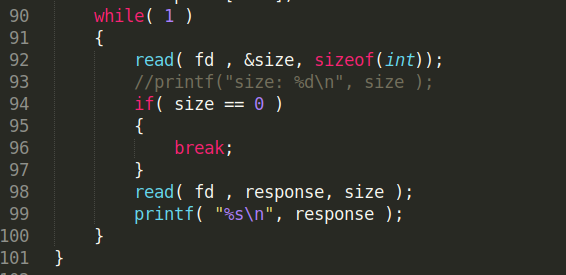
\includegraphics[width=10cm]{send_data.PNG}
    
\end{figure}

\subsection{ Preventing Multiple Instantiation }
I used temporary file for preventing multiple instantiation of server. At the beginning of the program server check if there is a file with name of "15104404\textunderscore temp". If the file exists it prints an error message and terminate. If no file with the specified name it creates the file. And at the end of the program it removes the file temporarily created file.




\section{Which requirements I achieved}

\begin{itemize}
  \item The report prepeared via latex. (latex folder is in the homework)
  \item All synchronization problems solved with condition variables and mutexes.
  \item No input file modified.
  \item I have a make file. It only compiles files
  \item The server run as a single instance.
  \item Server is a deamon. (No possible double instantiation)
  \item I loaded csv in array form (dynamically allocated).
  \item Thread pool works as expected.
  \item The threads  sleeps additionally 0.5 seconds to simulate intensive database execution.
  \item All queries works properly. ( select star, select distinct, select column, update  )
  \item On SIGINT all processes terminated. But there are some memory leak.
  \item No warning with -W flag
  \item If the required command line arguments are missing/invalid, The program prints usage information and exit.
  \item No busy waiting.
  \item The make file only compiles the program.
\end{itemize}


\section{Which Requirements I Fail:}

\begin{itemize}
  \item Memory leak on server.
  \item SQL commands are not perfectly parsed. Some valid commands might not be parsed.
\end{itemize}

\section{Notes:}

\begin{itemize}
  \item For creating demon and creating sockets I used some code from internet. But for deamons there are already samole code in course slides.

\end{itemize}

Screen soot for the log file of server as follows:

\begin{figure}[htp]
    \centering
    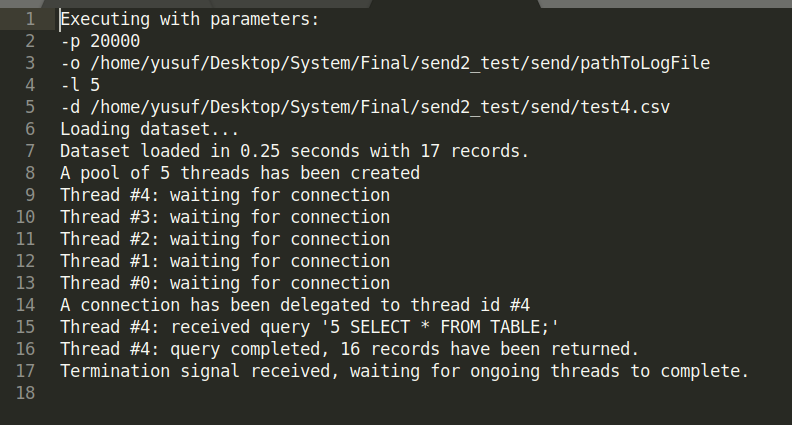
\includegraphics[width=11cm]{output.PNG}
    
\end{figure}

\end{document}
